\section{PDEs from Variational Principles}

Consider functionals of functions
\[
    \functiondomain{\vb{y}}{\RR^{m}}{\RR^{n}}
\]
for \(m > 1\), and functionals of the form
\[
    F\bqty{\vb{y}} = \int_{V} \dd[m]{\vb{x}} f\pqty{\vb{y}, \grad \vb{y}, \vb{x}}
\]
where \(V \subseteq \RR^m\), and the gradient is a \(m \times n\) matrix.

Similarly, we studying the variation of the functional, but here we using divergence theorem instead of a one-dimensional integration by parts. This leads to a generalisation of Euler--Lagrange equations, provided that the boundary conditions implies that the boundary term (surface integral) all vanishes.

\subsection{Minimal Surfaces}

Consider surfaces spanning a closed curve \(\mathcal{C}\) in \(\RR^3\). Which surface has the minimal area?

\begin{figure}[ht!]
    \centering
    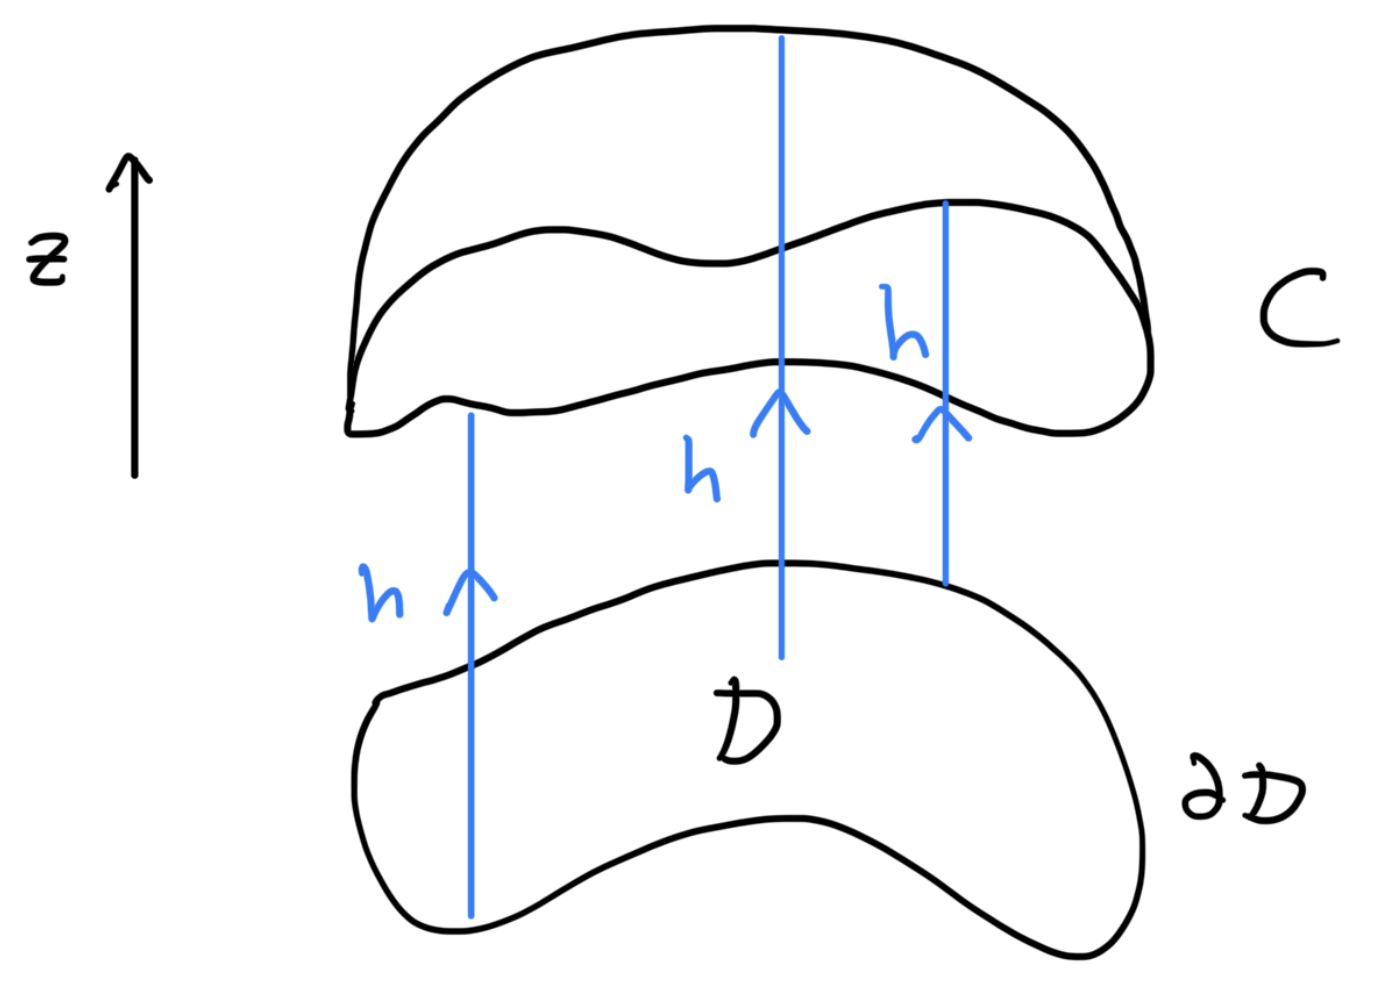
\includegraphics[width=0.5\linewidth]{fig/minimal-surface.png}
    \caption{Minimal Surface Problem}
    \label{fig:minimal-surface}%
\end{figure}

\begin{example}[Derivation of Minimal Surface Equation]
    For simplicity, we consider surfaces of the form
    \[
        z = h \pqty{x, y}
    \]
    for \(\pqty{x, y} \in \mathcal{D}\), with \(\mathcal{C}\) being the boundary of the graph, i.e. maps \(\partial \mathcal{D}\) to \(\mathcal{C}\). In particular, this means that \(h\) is fixed on \(\partial \mathcal{D}\). This is shown in \autoref{fig:minimal-surface}.

    This allows us to parameterise surface with \(\pqty{x, t}\), with
    \[
        \vb{x} \pqty{x, y} = \pqty{x, y, h\pqty{x, y}}.
    \]

    Hence,
    \[
        \pdv{\vb{x}}{x} = \pqty{1, 0, h_x} \qand \pdv{\vb{x}}{y} = \pqty{0, 1, h_y}.
    \]

    Then we have
    \[
        \dd{\vb{S}} = \pdv{\vb{x}}{x} \cross \pdv{\vb{x}}{y} \dd{x} \dd{y} = \pqty{-h_x, -h_y, 1} \dd{x} \dd{y}
    \]
    and hence
    \[
        \dd{A} = \sqrt{1 + h_x^2 + h_y^2} \dd{x} \dd{y}.
    \]

    Hence, the surface has area
    \begin{equation}
        \label{eq:area-functional}%
        A \bqty{h} = \iint_{\mathcal{D}} \sqrt{1 + h_x^2 + h_y^2} \dd{x} \dd{y}.
    \end{equation}

    Varying \(h\) to \(h + \var{h}\), we have
    \begin{align*}
        \var{A} &= \iint_{\mathcal{D}} \frac{h_x \pqty{\delta h}_x + h_y \pqty{\delta h}_y}{\sqrt{1 + h_x^2 + h_y^2}} \dd{x} \dd{y} \\
        &= \iint_{\mathcal{D}} \Bqty{\pqty{\frac{h_x \var{h}}{\sqrt{\cdots}}}_x + \pqty{\frac{h_x \var{h}}{\sqrt{\cdots}}}_y - \bqty{\pqty{\frac{h_x}{\sqrt{\cdots}}}_x + \pqty{\frac{h_y}{\sqrt{\cdots}}}_y} \var{h}} \dd{x} \dd{y}.
    \end{align*}
    
    Using Green's Theorem on a plane for the boundary term, we see the first divergence term vanishes, since \(\var{h} = 0\) on \(\partial \mathcal{D}\). Hence, \(A\) is extremisms if \(\var{A} = 0\) for all \(\var{h}\), and hence
    \[
        \pqty{\frac{h_x}{\sqrt{1 + h_x^2 + h_y^2}}}_x + \pqty{\frac{h_y}{\sqrt{1 + h_x^2 + h_y^2}}}_y = 0.
    \]

    This simplifies to
    \[
        \pqty{1 + h_y^2} h_{xx} + \pqty{1 + h_x^2} h_{yy} - 2 h_x h_y h_{xy} = 0,
    \]
    which is the \emph{minimal surface equation}. This is a second-order non-linear PDE for \(h = h\pqty{x, y}\).
\end{example}

If \(\abs{h_x}, \abs{h_y} \ll 1\), then the equation simplifies to \(h_{xx} + h_{yy} = 0\) which is Laplace's equation.

Note that one particular solution is when the second derivative of \(h\) is all zero, i.e., when
\[
    h = Ax + By + C
\]
describing a plane. But does this satisfy the boundary condition? This only satisfies the boundary conditions if the curve \(\mathcal{C}\) is planar.

\begin{example}[Solution when the Surface is Cylindrically Symmetric]
    We look for solutions that are surfaces of revolution (about \(z\)-axis), i.e. \(h\pqty{x, y} = z\pqty{r}\) where \(r = \sqrt{x^2 + y^2}\). Then this reduces to
    \[
        r z'' + z' + \pqty{z'}^3 = 0
    \]
    which is an ODE, but still hard to solve.
    
    Instead, we could put this back into \autoref{eq:area-functional}, then
    \[
        \dd{x} \dd{y} = r \dd{r} \dd{\phi}
    \]
    and hence
    \[
        A\bqty{z} = 2 \pi \int r \sqrt{1 + z'^2} \dd{r},
    \]
    in this case assuming that the region \(\mathcal{D}\) is a circle with radius \(R\).
    
    Now we optimise w.r.t. \(z\pqty{r}\), and there is no dependence on \(z\), giving a first integral, giving a solution of the form
    \[
        r = r_0 \cosh \pqty{\frac{z - z_0}{r_0}},
    \]
    which is a \emph{catenoid}, as in \autoref{fig:catenoid}.
\end{example}

\begin{figure}[ht!]
    \centering
    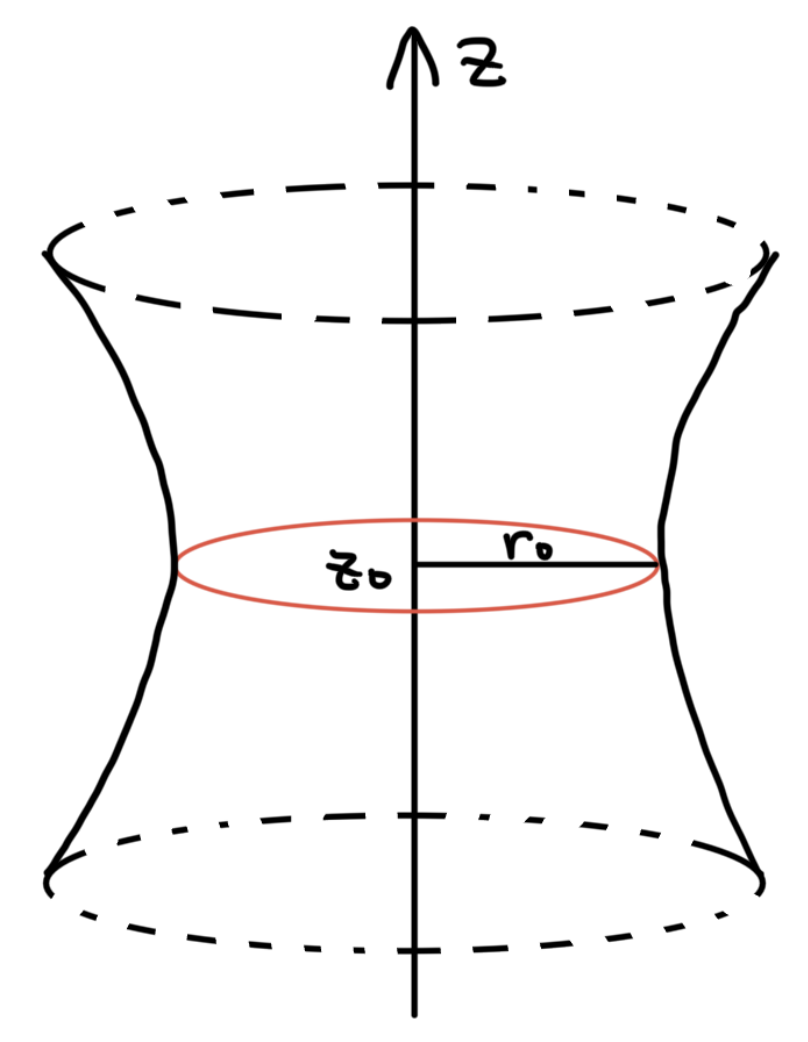
\includegraphics[width=0.4\linewidth]{fig/catenoid.png}
    \caption{Catenoid}
    \label{fig:catenoid}
\end{figure}

Another example is a \emph{helicoid} which is in Example Sheet 2.

\subsection{Vibrating String}

\begin{example}[Derivation of Wave Equation]
    A string with tension \(T\) and mass per unit length \(\rho\) has kinetic energy
    \[
        \text{K.E.} = \frac{1}{2} \rho \int_{0}^{a} \dot{y} \pqty{t, x}^2 \dd{x}
    \]
    and potential energy
    \[
        \text{P.E.} = \frac{1}{2} T \int_{0}^{a} y' \pqty{t, x}^2 \dd{x}.
    \]
    
    Then the action \(I\) is given by
    \begin{equation}
        I \bqty{y} = \frac{1}{2} \int_{t_0}^{t_1} \dd{t} \int_{0}^{a} \dd{x} \pqty{\rho \dot{y}^2 - T y'^2}.
    \end{equation}
    
    Varying \(y\) to \(y + \var{y}\), we get
    \begin{align*}
        \var{I} &= \int_{t_0}^{t_1} \dd{t} \int_{0}^{a} \dd{x} \pqty{p \dot{y} \var{\dot{y}} - T y' \var{y}'} \\
        &= \int_{t_0}^{t_1} \dd{t} \int_{0}^{a} \dd{x} \Bqty{\pdv{t} \pqty{\rho \dot{t} \var{y}} - \pdv{x} \pqty{T y' \var{y}} + \pqty{- \rho \ddot{y} + T y''} \var{y}}.
    \end{align*}
    
    The boundary terms integrate to zero, if \(\var{y} = 0\) on the boundary. So \(\var{I} = 0\) iff we have
    \[
        \ddot{y} - v^2 y'' = 0
    \]
    where \(v = \sqrt{\flatfrac{T}{\rho}}\). This is the \emph{wave equation}, and its one-dimensional solution is
    \[
        y\pqty{t, x} = f \pqty{x - vt} + g \pqty{x + vt}
    \]
    as seen in \textit{Differential Equations}.
\end{example}

\subsection{Action for Maxwell's Equations}

Consider electric and magnetic fields \(\vb{E} \pqty{t, \vb{x}}\) and \(\vb{B} \pqty{t, \vb{x}}\). Two of Maxwell's Equations are
\begin{subequations}
    \begin{equation}
        \label{eq:b-curlless}%
        \div \vb{B} = 0
    \end{equation}
    \begin{equation}
        \label{eq:faraday}%
        \curl \vb{E} = - \pdv{t} \vb{B}.
    \end{equation}
\end{subequations}

\autoref{eq:b-curlless} tells us that \(\vb{B} = \curl \vb{A}\) for some \(\vb{A} \pqty{t, \vb{x}}\). Then putting this into \autoref{eq:faraday}, gives us
\[
    \curl \pqty{\vb{E} + \pdv{t} \vb{A}} = \vb{0}
\]
and hence
\[
    \vb{E} = - \grad \phi - \pdv{t} \vb{A}
\]
for some \(\phi\pqty{t, \vb{x}}\). They are called the \emph{magnetic potential} and \emph{electric potential} respectively.

\begin{example}[Deriving the Remaining Two Maxwell's Equations]
    The actions is, in fact, a functional of \(\vb{A}\) and \(\phi\), in the form
    \[
        I\bqty{\vb{A}, \phi} = \int \dd{t} \iiint \dd[3]{\vb{x}} \Bqty{\frac{1}{2} \epsilon_0 \vb{E}^2 - \frac{1}{2 \mu_0} \vb{B}^2 + \vb{A} \vdot \vb{j} - \phi \rho}
    \]
    where \(\vb{j}\pqty{t, \vb{x}}\) is the \emph{current density}, and \(\rho\pqty{t, \vb{x}}\) is the \emph{charge density}.
    
    We vary \(\vb{A}\) and \(\phi\). We have
    \begin{align*}
        \var{I} &= \int \dd{t} \iiint \dd[3]{\vb{x}} \Bqty{\epsilon_0 \vb{E} \vdot \pqty{- \grad \var{\phi} - \pdv{t} \var{\vb{A}}} - \frac{1}{\mu_0} \vb{B} \vdot \pqty{\curl \var{\vb{A}}} + \var{\vb{A}} \vdot \vb{j} - \var{\phi} \rho} \\
        &= \int \dd{t} \iiint \dd[3]{\vb{x}} \Bqty{\epsilon_0 \vb{E} \bqty{- \div \pqty{\vb{E} \var{\phi}} + \pqty{\div \vb{E}} \var{\phi} - \pdv{t} \pqty{\vb{E} \vdot \var{\vb{A}}} + \pqty{\pdv{t} \vb{E}} \vdot \var{\vb{A}}}} \\
        &\phantom{=} \Bqty{- \frac{1}{\mu_0} \bqty{\pdv{x_j} \pqty{\levicivita_{ijk} B_i \var{A_k} - \pqty{\levicivita_{ijk} \pdv{x_j} B_i} \var{A_k}}} + \var{\vb{A}} \vdot \vb{j} - \var{\phi} \rho} \\
        &= \text{boundary terms} + \int \dd{t} \iiint \dd[3]{\vb{x}} \Bqty{\pqty{\epsilon_0 \div \vb{E} - \rho} \var{\phi} + \pqty{- \frac{\curl \vb{B}}{\mu_0} + \epsilon_0 \pdv{t} \vb{E} + \vb{j}} \vdot \var{\vb{A}}}.
    \end{align*}
    
    Assuming boundary terms vanish, we can read that \(\var{I}\) is zero for arbitary \(\var{\vb{A}}\) and \(\vb{\phi}\), if and only if
    \begin{subequations}
        \begin{equation}
            \div \vb{E} = \frac{\rho}{\epsilon_0}
        \end{equation}
        \begin{equation}
            \curl \vb{B} = \mu_0 \pqty{\vb{j} + \epsilon_0 \pdv{t} \vb{E}}
        \end{equation}
    \end{subequations}
    giving the remaining Maxwell's equations.
\end{example}